\chapter{Related Work}\label{chapter:related_work}
This work is not the first to explore the area of code generation and compilation for regular expressions. In 2008, \citet{firejpaper} implemented FIRE/J (Fast Implementation of Regular Expressions for Java), which is a portable POSIX-compatible Java regular expression library that focuses on providing maximum regex matching speed. Their implementation converted the regular expression into a determinstic finite automata (DFA) compiled directly into Java source code or JVM bytecode.

Figure \ref{fig:firejpaper} shows the bytecode generated by FIRE/J. The bytecode is similar to our generated LLVM code structure discussed in Chapter \ref{chapter:related_work}. The algorithm lists each DFA state starting from the initial state, and then the input characters are checked against the transition rules of the DFA states. If a character does not satisfy the selected state, the match fails. Otherwise, the code jumps to the next state. When the input is finished, the code checks if the state is terminal, then the match succeeds. Otherwise, it fails.

While their approach is similar to ours, there are a few differences between theirs and ours (1) their use-case is to be used as a generic java library, while ours is usage as a sub-engine inside a database. (2) The execution and compilation speed of LLVM compiler infrastructure is far superior to traditional JVM bytecode that Azul JVM implementation based on LLVM is 5 to 250 percent faster than Oracle's HotSpot Java platform \cite{azul}.

\begin{figure}[htbp]
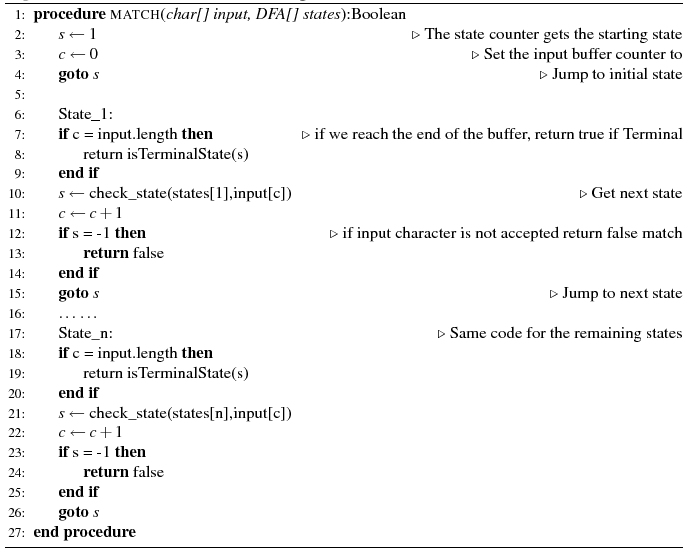
\includegraphics[width=\textwidth]{imgs/alg-byte-firej.png}
\caption{Bytecode generated by FIRE/J \cite{firejpaper}.}\label{fig:firejpaper}
\end{figure}

PCRE2 \cite{pcre2} is a regular expressions matching library for the C programming language. This library translates the patterns into bytecode that its interpreter can execute. In 2016, \citet{pcre2_jit} developed a new backtracking-based matching algorithm for PCRE2 called \textit{static-backtracking} and a JIT compiler for PCRE2 called \textit{PCRE-JIT}.

The static backtracking algorithm generates machine code from the Abstract Syntax Tree (AST). The AST representation provides more information about the pattern's structure and allows the engine to optimize matching and backtracking simultaneously rather than focus on matching. The PCRE-JIT compiler transforms PCRE bytecode into low-level intermediate representation (LIR) language of the Stackless Just-In-Time Compiler (SLJIT), translating it into machine code. In Chapter \ref{chapter:evaluation}, We compare our DFA-based engine performance to that of PCRE-JIT.

ReJit \cite{rejit} is a prototype of a non-backtracking, just-in-time, SIMD-able regular expression engine. ReJit generates tailored machine code to match each regular expression and passes it to a JIT compiler that identifies what CPU instructions are available at run-time and creates efficient code for performance-critical areas.

Despite being based on Finite Automaton, It supports most regular expression capabilities (including some that RE2 does not, such as back-references). Backtracking is used locally to handle back-references and not as a general algorithm.

When Matching complex regular expressions, Most engines will try to match the regular expressions from the start, which might be wasteful. ReJit, on the other hand, tries to find the easy section of the regular expression first and then complete the match from there. E.g. for the pattern \texttt{\textbf{[0-9]{3,10}\%foo\%[A-Za-z]}}, it generates code that first searches for \texttt{\textbf{foo}} and then proceeds backward and forward to match the entire phrase.

ReJit is a promising engine but is still a work-in-progress. It currently only supports \texttt{\textbf{X86}} CPU architecture. It is also not in active development since 2015 (time of the last commit \footnote{\url{https://github.com/coreperf/rejit/commit/36855db0644d6f3dbad69dc65cf002c81510ea19}}).

\citet{simdregextpch} in their paper SIMD-Accelerated Regular Expression Matching, presented the design and implementation of SIMD-vectorized regular expression matching for filtering DBMSs string columns. 

Their approach processes multiple-input strings in a data-parallel way that avoids reading the strings in lockstep without branching to exploit scenarios when some strings are accepted or rejected early by inspecting the first few characters. Their approach achieved up to $2x$ speedup on a mainstream CPU and $5x$ on the Xeon Phi co-processor using common string lengths.


\citet{parabixorg} introduced Parabix (Parallel Bit Streams), a generic framework and toolkit describing the software toolchain and run-time support that enables applications to use modern SIMD instructions for high-performance text processing.

Parabix exploits data-level parallelism of wide SIMD registers to implement parallel bit streams through bitwise data parallelization. In 2014, \citet{parabixregexnew} developed a new algorithm and compiler that utilized using bitwise data parallelism for regular expression matching. The algorithm represents a general solution to the problem of regular expression matching utilizing parallel bit streams. The prototype compiler consisted of a toolchain that compiled a regular expression to bit-parallel streams. The compiler compiles the bit-stream to highly efficient SIMD C++ code, then compiled to machine code. The prototype did not support Unicode. It only supported ASCII.

In 2015, \citet{parabix} unified the toolchain into a single executable compiler that is highly efficient Unicode-capable and is dynamically compiled (JITed) using the LLVM compiler infrastructure. Compared to other Unicode-capable regular expression search tools, performance evaluations reveal asymptotic performance advantages of more than 10X. At the same time, the overhead of dynamic compilation approaches restricts the benefits to rather large input files.